\documentclass[aspectratio=169]{beamer}

\usetheme{Madrid}

\usecolortheme{seahorse}

\usepackage{graphicx}

\usepackage{booktabs}

\usepackage{amsmath}

\usepackage{xcolor}

\title[Chapter 2: Numerical Summaries]{\textbf{Chapter 2: Describing Distributions with Numbers}}

\subtitle{School of Mathematical and Computational Sciences \\ University of Prince Edward Island}

\author{Ali Raisolsadat}

\date{Part I: Exploring Data}

\begin{document}

% =============================================================
% PART I: INTRODUCTION & OBJECTIVES
% =============================================================

% SLIDE 1
\begin{frame}
 \titlepage
\end{frame}


% SLIDE 2
\begin{frame}{The Limits of Human Perception}
\begin{itemize}
	\item In Chapter 1 we learned the first rule of modern data analysis: \textbf{always plot your data}.
	\item Visualizations (histograms, dotplots) allow our eyes to quickly spot shapes, trends, bimodal clusters and data entry errors.
	\item \textbf{The Problem:} Human eyes are subjective! 
	\begin{itemize}
		\item If you ask two scientists to point to the "center" of a skewed histogram, they will point to two different spots.
	\end{itemize}
	\item \textbf{The Solution:} We need to translate our visual descriptions - Shape, Outliers, Center and Spread (SOCS) - into objective, reproducible statistical summaries.
\end{itemize}
\end{frame}


% =============================================================
% PART II: MEASURING CENTER (MEAN & MEDIAN)
% =============================================================

% SLIDE 3
\begin{frame}{Measuring Center: What is "Typical"?}
 \begin{block}{Defining the Center}
When a biologist asks \emph{"What is the typical length of a pine needle?"} or \emph{"What is the normal number of flood events on the coast?"}, they are asking for a measure of \textbf{center}.
\end{block}

\vspace{0.3cm}

Statistics gives us two primary ways to define "typical" and they behave very differently depending on the shape of the data:

\begin{itemize}
	\item The \textbf{Mean} ($\bar{x}$)
	\item The \textbf{Median} ($M$)
\end{itemize}
\end{frame}

% SLIDE 4
\begin{frame}{The Mean ($\bar{x}$)}
The most commonly reported measure of center is the ordinary arithmetic average or \textbf{mean}. To find it, add all values together and divide by the number of observations ($n$).

\vspace{0.2cm}

If the $n$ observations are $x_1, x_2, \dots, x_n$, their sample mean is
$$ \bar{x} = \frac{x_1 + x_2 + \dots + x_n}{n} $$
We use the uppercase Greek letter sigma ($\sum$) to mean "add them all up". So the compact formula is
$$ \bar{x} = \frac{1}{n} \sum x_i $$
\end{frame}

% SLIDE 5
\begin{frame}{Notation Note: Sample vs. Population}
\begin{itemize}
	\item The subscripts ($x_i$) just keep the $n$ observations distinct; they do not necessarily indicate chronological order.
	\item The bar over the $x$ indicates the mean of all the $x$-values.
\end{itemize}
\vspace{0.3cm}
\begin{alertblock}{Important Distinction}
We use $\bar{x}$ to represent the mean of a \emph{sample} of data. Later in the course, we will use the Greek letter $\mu$ (mu) to represent the theoretical mean of an entire \emph{population}. Whenever you see $\bar{x}$ in a paper, the authors are discussing sample data.
\end{alertblock}
\end{frame}


% SLIDE 6
\begin{frame}{Example 2.3: Mean of Pine Needle Lengths}
Let's find the mean of the needle length for a sample of $n = 15$ Aleppo pine needles. The sample lengths are given in the table below.
\vspace{0.2cm}
\begin{table}
\centering
\scriptsize
\begin{tabular}{cc|cc|cc}
\toprule
\textbf{Obs ($i$)} & \textbf{$x_i$ (cm)} & \textbf{Obs ($i$)} & \textbf{$x_i$ (cm)} & \textbf{Obs ($i$)} & \textbf{$x_i$ (cm)} \\
\midrule
1 & 7.2 & 6 & 9.0 & 11 & 10.2 \\
2 & 7.6 & 7 & 9.0 & 12 & 10.9 \\
3 & 8.5 & 8 & 9.3 & 13 & 11.3 \\
4 & 8.5 & 9 & 9.4 & 14 & 12.1 \\
5 & 8.7 & 10 & 9.4 & 15 & 12.8 \\
\bottomrule
\end{tabular}
\end{table}
\end{frame}

% SLIDE 7
\begin{frame}{Example 2.3: Calculating the Mean}

\textbf{Step 1: Sum the values ($\sum$)}
$$ \sum_{i=1}^{15} x_i = 7.2 + 7.6 + \dots + 12.8 = 143.9 \text{ cm} $$

\textbf{Step 2: Divide by $n$}
$$ \bar{x} = \frac{1}{n} \sum_{i=1}^{15} x_i = \frac{143.9}{15} \approx 9.59 \text{ cm} $$

\vspace{0.3cm}

\emph{Takeaway:} The he formula reminds us of a critical fact that the mean mathematically incorporates the actual numerical value of every single observation.
\end{frame}

% SLIDE 8
\begin{frame}[fragile]{Example 2.3: Calculating the Mean in R}
We can use R to find the mean instantly.

\vspace{0.1cm}

\begin{block}{R Code}
\begin{verbatim}
# Create a vector of the 15 pine needle lengths
pine_needles <- c(7.2, 7.6, 8.5, 8.5, 8.7, 9.0, 9.0, 9.3, 
                  9.4, 9.4, 10.2, 10.9, 11.3, 12.1, 12.8)

# Calculate the mean
mean(pine_needles)
\end{verbatim}
\end{block}
\textbf{Output:}
\texttt{[1] 9.593333}
\end{frame}

% SLIDE 9
\begin{frame}{The Median ($M$)}
\begin{itemize}
	\item The \textbf{median} is the exact geometric midpoint of a distribution.
	\item It is the 50th percentile. This is the number such that exactly half (50\%) of the observations are smaller and the other half are larger.
\end{itemize}

\vspace{0.3cm}

\textbf{How to locate the median ($M$)}
\begin{enumerate}
	\item \textbf{Sort} all observations in order from smallest to largest.
	\item If $n$ is \textbf{odd}, the median is located at position \textbf{$\frac{n+1}{2}$} of the ordered data.
   	 \item If $n$ is \textbf{even}, this lands between two numbers, and you take their average.
\end{enumerate}
\end{frame}

% SLIDE 10
\begin{frame}[fragile]{Software Note: The Median in R}
\begin{block}{Calculating the Median}
In R, the median is calculated using the simple \texttt{median()} function.
\end{block}

\vspace{0.3cm}

Unlike calculating by hand where we must sort the data first, R handles the sorting, locating and averaging (if $n$ is even) automatically behind the scenes. 
\end{frame}

% SLIDE 11
\begin{frame}{Example 2.1: Finding the Median (Odd $n$)}
What is the median length for our $15$ Aleppo pine needles?
\vspace{0.cm}
\begin{enumerate}
	\item \textbf{Sort the data:} \\
	\begin{table}
	\centering
	\scriptsize
		\begin{tabular}{cc|cc|cc}
		\toprule
		\textbf{Obs ($i$)} & \textbf{$x_i$ (cm)} & \textbf{Obs ($i$)} & \textbf{$x_i$ (cm)} & \textbf{Obs ($i$)} & \textbf{$x_i$ (cm)} \\
		\midrule
		1 & 7.2 & 6 & 9.0 & 11 & 10.2 \\
		2 & 7.6 & 7 & 9.0 & 12 & 10.9 \\
		3 & 8.5 & 8 & 9.3 & 13 & 11.3 \\
		4 & 8.5 & 9 & 9.4 & 14 & 12.1 \\
		5 & 8.7 & 10 & 9.4 & 15 & 12.8 \\
		\bottomrule
		\end{tabular}
	\end{table}
    \item \textbf{Locate the median:} \\
    $$ \text{Location} = \frac{n+1}{2} = \frac{15+1}{2} = 8 $$
    \item \textbf{Find the middle:} he 8th observation in the sorted list is 9.3 cm.
\end{enumerate}
 
\vspace{0.1cm}

\textbf{Result:} Median ($M$) = $9.3\text{ cm}$.
\end{frame}

% SLIDE 12
\begin{frame}[fragile]{Example 2.1: Finding the Median in R (Odd $n$)}
\begin{block}{R Code}
\begin{verbatim}
# Using our pine_needles vector from earlier
median(pine_needles)
\end{verbatim}
\end{block}
\textbf{Output:}
\texttt{[1] 9.3}
\end{frame}

% SLIDE 13: Example 2.2: Finding the Median (Even n)
\begin{frame}{Example 2.2: Finding the Median (Even $n$)}
Now we have the lengths of $18$ needles from the Torrey pine species.
\vspace{0.1cm}
\begin{enumerate}
    \item \textbf{Sort the data:} \\
    {\small 21.2, 21.6, 21.7, 23.1, 23.7, 24.2, 24.2, 25.5, 26.6,\\
	       26.8,28.9,29.0, 29.7, 29.7, 30.2, 32.5, 33.7, 33.7}
    \item \textbf{Locate the median:}
    $$ \text{Location} = \frac{n+1}{2} = \frac{18+1}{2} = 9.5 $$
    \item \textbf{Find the middle:} Location 9.5 means exactly halfway between the 9th and 10th observations $$\frac{26.6 + 26.8}{2}$$.
\end{enumerate}
\vspace{0.2cm}
\textbf{Result:} Median ($M$) = $26.7\text{ cm}$
\end{frame}

% SLIDE 14
\begin{frame}[fragile]{Example 2.2: Finding the Median in R (Even $n$)}
 \begin{block}{R Code}
 \begin{verbatim}
# Create a vector of the 18 Torrey pine needle lengths
torrey_needles <- c(21.2, 21.6, 21.7, 23.1, 23.7, 24.2, 
                  24.2, 25.5, 26.6, 26.8, 28.9, 29.0, 
                  29.7, 29.7, 30.2, 32.5, 33.7, 33.7)

# Calculate the median
median(torrey_needles)
\end{verbatim}
\end{block}
\textbf{Output:}
\texttt{[1] 26.7}
\end{frame}

% =============================================================
% PART III: COMPARING MEAN & MEDIAN (RESISTANCE)
% =============================================================


% SLIDE 15
\begin{frame}{Comparing Mean and Median: Resistance}
If both the mean and the median measure the ``center'' why do we need both? 

\textbf{Because they react differently to extreme biology.}
\vspace{0.3cm}
\begin{itemize}
	\item A statistical measure is called \textbf{resistant} (or robust) if it is not strongly influenced by a few extreme observations (outliers).
	\item \textbf{The Median is Resistant:} It is influenced \emph{only} by the total number of data points and the physical order of the numbers.
	\item \textbf{The Mean is Non-Resistant:} Because the mean adds up the numerical value of every single observation, it cannot resist the pull of extreme outliers.
\end{itemize}
\end{frame}

% SLIDE 16
\begin{frame}{Example: The ``Long-Hauler'' Patient}
Patients tracking days for Heart Rate Variability (HRV) to return to baseline.
\vspace{0.2cm}
\begin{columns}[T]
\begin{column}{0.48\textwidth}
\textbf{Normal Sample} \\
	Sorted: 4, 6, 7, 8, 9 \\
	\vspace{0.2cm}
	\begin{itemize}
		\item \textbf{Median ($M$):} 7 days
		\item \textbf{Mean ($\bar{x}$):} 6.8 days
	\end{itemize}
	\emph{(For symmetric data, they are very close together).}
	\end{column}
	
	\begin{column}{0.48\textwidth}
	\textbf{Sample with Outlier} \\
	Sorted: 4, 6, 7, 8, \textbf{45} \\
	\vspace{0.2cm}
	\begin{itemize}
		\item \textbf{Median ($M$):} 7 days \\ \emph{(Did not change!)}
		\item \textbf{Mean ($\bar{x}$):} 14.0 days \\ \emph{(Drastically pulled right!)}
     	 \end{itemize}
  	 \end{column}
\end{columns}
\end{frame}

% SLIDE 17
\begin{frame}{Visualizing Resistance to Outliers}
\begin{center}
	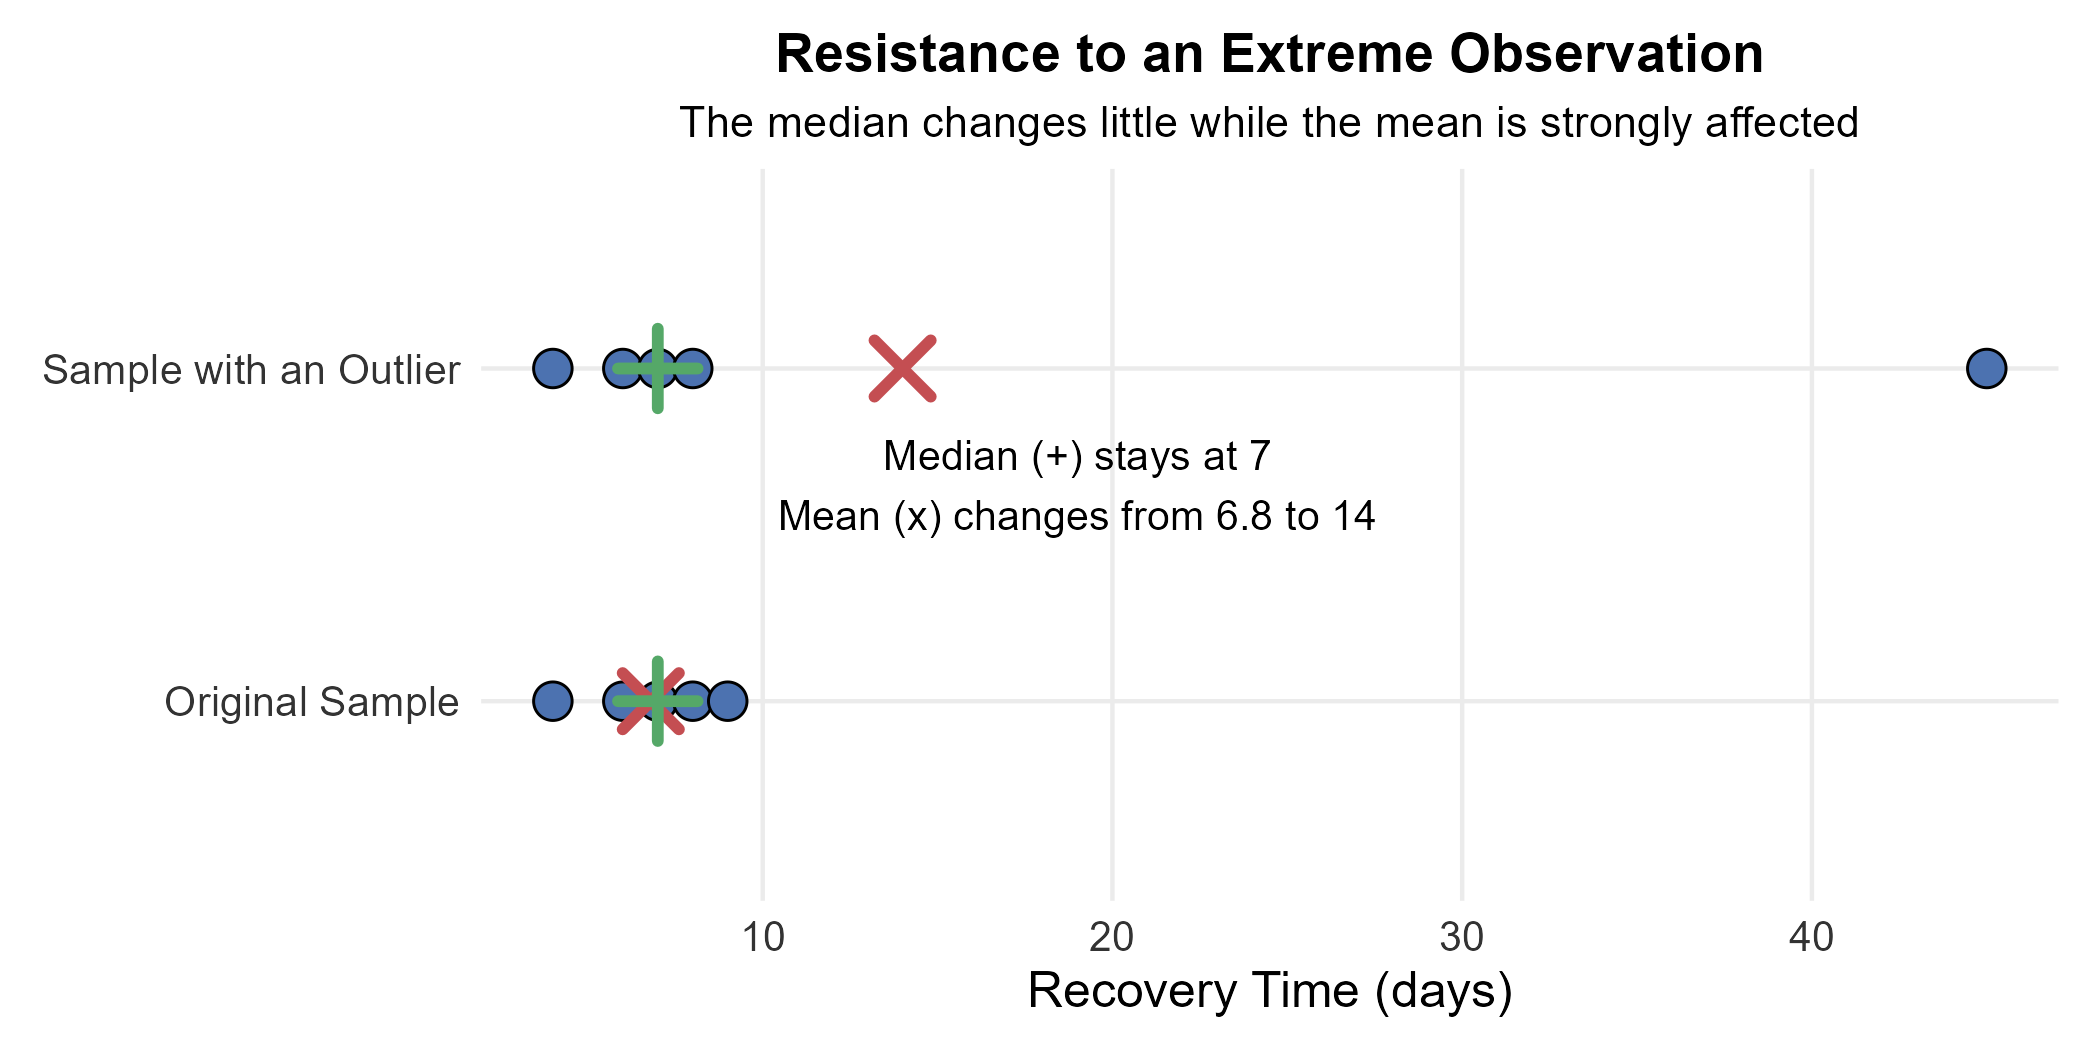
\includegraphics[width=0.65\textwidth]{fig_ch2_resistance.png}
\end{center}
\vspace{0.1cm}
\begin{itemize}
	\item \textbf{The Median is Resistant:} Changing the largest value does not change the physical midpoint.
	\item \textbf{The Mean is Non-Resistant:} The massive outlier acts like a heavy weight on the scale, dragging the mean toward it.
\end{itemize}
\end{frame}

% SLIDE 18
\begin{frame}{Shape Determines the Center}
Because of resistance, the shape of your distribution dictates how the mean and median will relate to each other:
\vspace{0.2cm}
\begin{table}
\centering
\small
\begin{tabular}{lp{6cm}}
\toprule
\textbf{Shape (Histogram)} & \textbf{Mathematical Relationship} \\
\midrule
\textbf{Symmetric} & Mean $\approx$ Median (Both sit in the center) \\
\textbf{Skewed Right} & Mean $>$ Median (Extreme high values pull mean to the right) \\
\textbf{Skewed Left} & Mean $<$ Median (Extreme low values drag mean to the left) \\
\bottomrule
\end{tabular}
\end{table}
\end{frame}

% SLIDE 19
\begin{frame}{Example: Viral Load and Skewness}
\begin{block}{Question}
The following illustrative viral load measurements were recorded in copies/mL. What are the mean and median and which better represents the centre of this strongly right-skewed dataset
\end{block}
\scriptsize
\begin{center}
\begin{tabular}{rrrrr}
120 & 140 & 160 & 180 & 200 \\
220 & 250 & 270 & 300 & 330 \\
360 & 400 & 450 & 520 & 600 \\
750 & 900 & 1300 & 2500 & 6000 \\
\end{tabular}
\end{center}
\end{frame}

% SLIDE 20
\begin{frame}{Visualizing Right-Skewed Data}
\begin{center}
	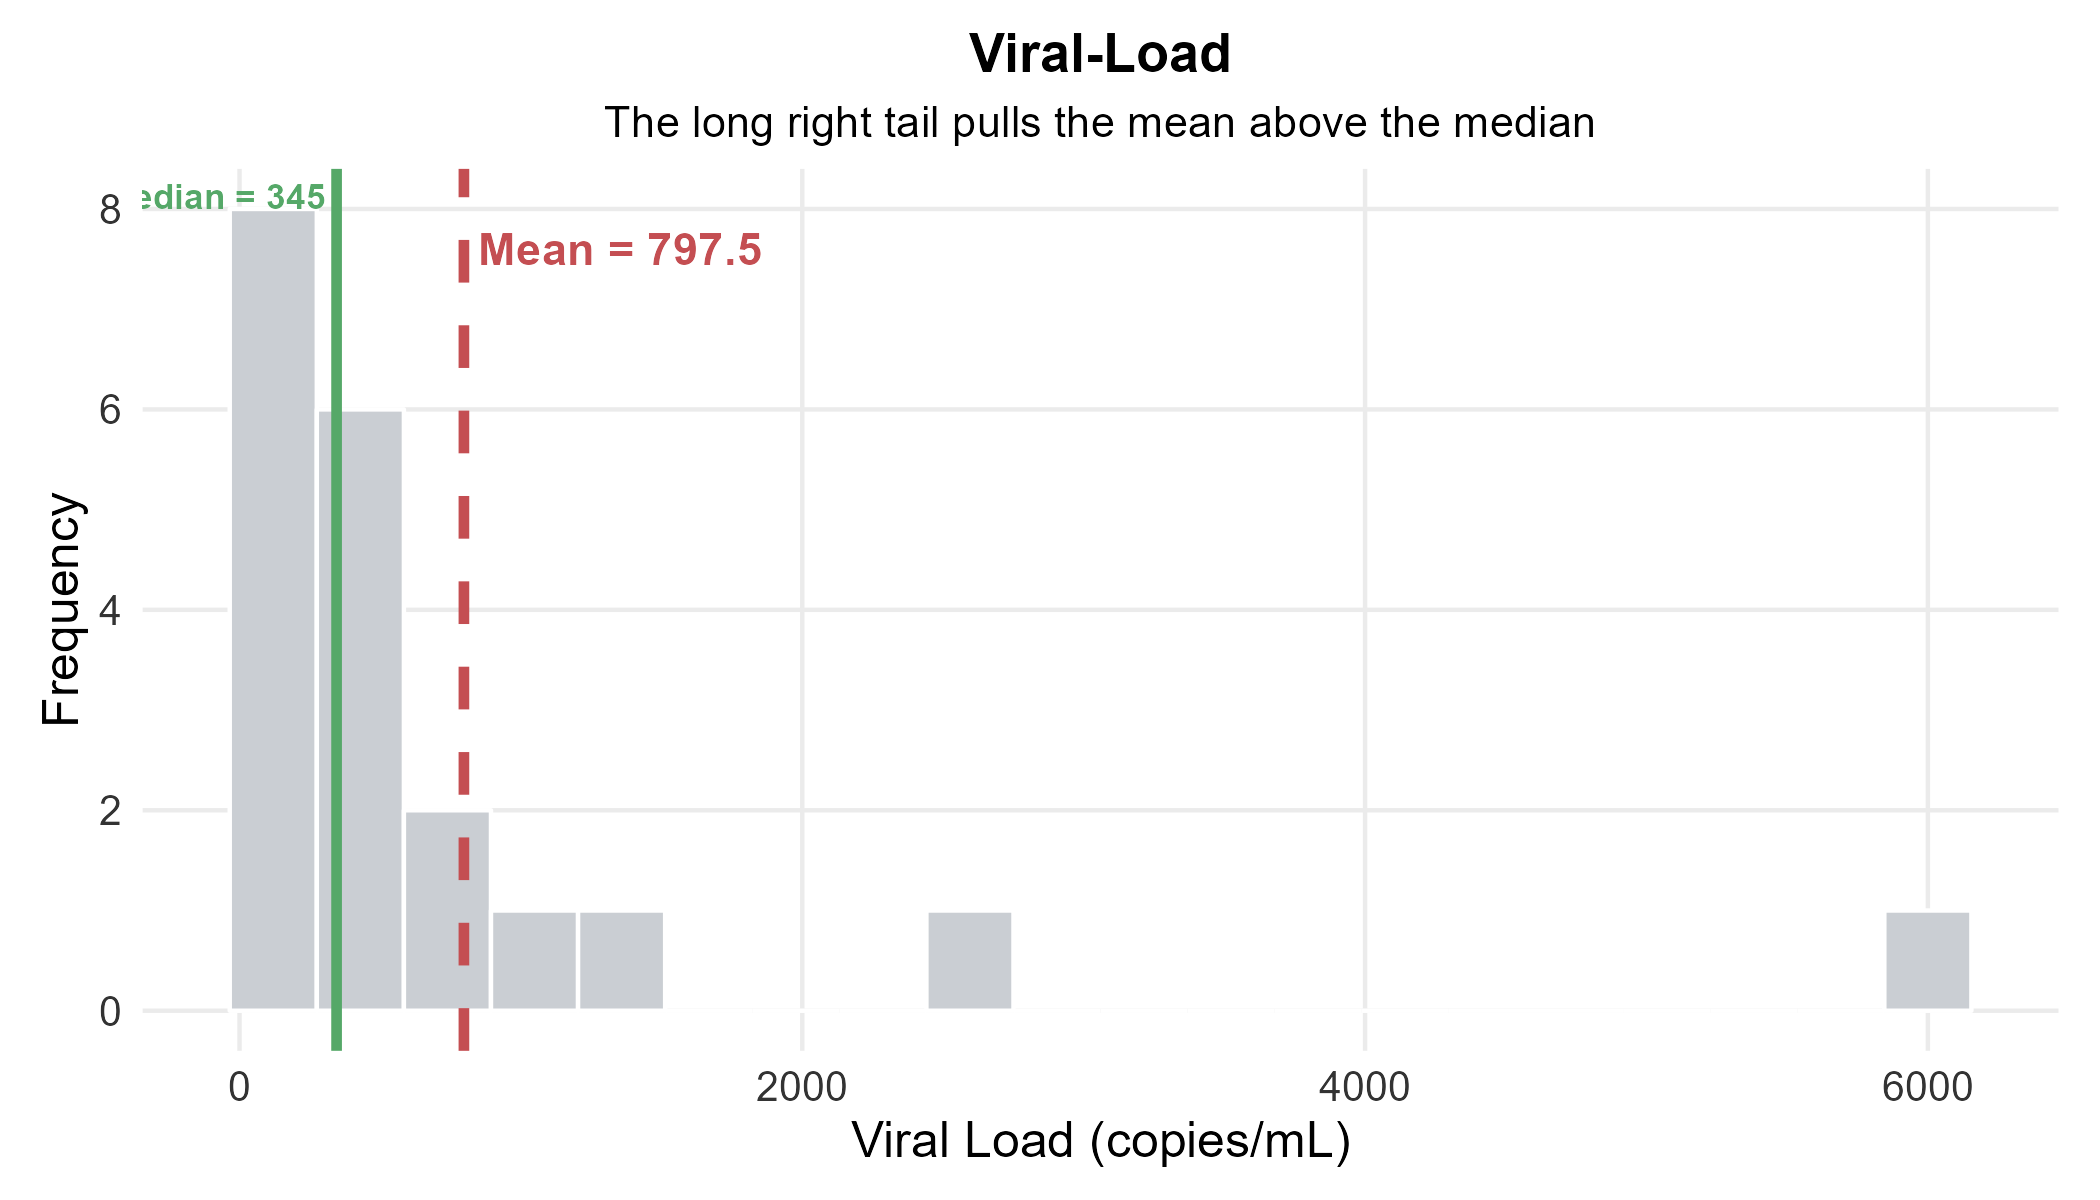
\includegraphics[width=0.75\textwidth]{fig_ch2_skewed_mean_median.png}
\end{center}
\end{frame}

% SLIDE 21
\begin{frame}{Biological Application: Survival Times}
\begin{itemize}
	\item Many biological variables (like viral loads or survival times) are \textbf{right-skewed}. 
	\item Most patients survive a typical duration, but a few ``super-responders'' survive for years, creating a long right tail.
	\item \textbf{Doctors} generally report the \emph{median} to patients because it represents the typical midpoint experience.
	\item \textbf{Hospitals} must calculate the \emph{mean} to project the total staffing and financial resources needed to cover all patient days.
	\item \emph{Takeaway:} Both measures measure ``center'' in different ways and both are scientifically useful!
\end{itemize}
\end{frame}

% =============================================================
% PART IV: MEASURING SPREAD (QUARTILES & BOXPLOTS)
% =============================================================

% SLIDE 22
\begin{frame}{Measuring Spread: Why Center Isn't Enough}
\begin{block}{Problem}
A biologist records the body weights of a sample of penguins in a colony. The median weight is \textbf{4.5 kg}. Is the median alone enough to describe the penguin weights?
\end{block}
\pause
\begin{itemize}
	\item The median of \textbf{4.5 kg} tells us about the center of the distribution.
	\item It does not tell us how much the individual penguin weights vary around that center.
	\item For example, are most penguins close to 4.5 kg, or do their weights range from about 2 kg to 8 kg?
	\item \textbf{Rule:} A measure of center should be accompanied by a measure of \textbf{spread} or variability.
\end{itemize}
\end{frame}

% SLIDE 23
\begin{frame}{The Quartiles ($Q_1$ and $Q_3$)}
Just as the median divides the data exactly in half, the quartiles divide the data into exactly four equal quarters.
\vspace{0.3cm}
\begin{itemize}
	\item \textbf{Quartile 1 ($Q_1$):} The median of the lower half of the data. Exactly \textbf{25\%} of the data falls below $Q_1$.
	\item \textbf{Quartile 3 ($Q_3$):} The median of the upper half of the data. Exactly \textbf{75\%} of the data falls below $Q_3$ (and 25\% is above it).
\end{itemize}
\end{frame}

% SLIDE 24
\begin{frame}{How to Calculate the Quartiles by Hand}
\begin{enumerate}
	\item Sort the data and find the overall Median ($M$).
	\item Locate the lower half of the data. The median of this lower half is $Q_1$.
	\item Locate the upper half of the data. The median of this upper half is $Q_3$.
	\item \emph{Note: If $n$ is odd, do not include the overall median in this lower half.}
\end{enumerate}
\end{frame}

% SLIDE 25
\begin{frame}{Example 2.5: Finding Quartiles (Odd $n$)}
Ordered Aleppo pine needle lengths ($n=15$)
\vspace{0.2cm}
\begin{table}
\centering
\small
\begin{tabular}{p{4cm}cp{4cm}}
\toprule
\textbf{Lower Half} & \textbf{Median} & \textbf{Upper Half} \\
\midrule
7.2, 7.6, 8.5, \textbf{8.5}, 8.7, 9.0, 9.0 & \textbf{9.3} & 9.4, 9.4, 10.2, \textbf{10.9}, 11.3, 12.1, 12.8 \\
\bottomrule
\end{tabular}
\end{table}
\begin{itemize}
	\item Overall Median ($M$) = \textbf{9.3 cm}.
	\item \textbf{$Q_1$:} The median of the 7 observations to the left. The middle of 7 is the 4th value $\rightarrow$ \textbf{8.5 cm}.
	\item \textbf{$Q_3$:} The median of the 7 observations to the right. The middle of 7 is the 4th value $\rightarrow$ \textbf{10.9 cm}.
	\item \emph{Notice: $Q_3$ would still be 10.9 cm even if the maximum needle was 50 cm! Quartiles are highly resistant.}
\end{itemize}
\end{frame}


% SLIDE 26
\begin{frame}[fragile]{Example 2.5: Finding Quartiles in R}
R provides several ways to find quartiles. The most common is the \texttt{summary()} function, which gives the quartiles, the extremes, and the mean all at once.
\vspace{0.3cm}
\begin{block}{R Code}
\begin{verbatim}
summary(pine_needles)
\end{verbatim}
\end{block}
\textbf{Output:}
\begin{verbatim}

   Min. 1st Qu.  Median    Mean 3rd Qu.    Max. 

  7.200   8.600   9.300   9.593  10.550  12.800 

 \end{verbatim}
\end{frame}


% SLIDE 27
\begin{frame}{Example 2.6: Finding Quartiles (Even $n$)}
Ordered Torrey pine needles length ($n=18$)
\vspace{0.2cm}
\begin{table}
\centering
\scriptsize
\begin{tabular}{p{4cm}cp{4cm}}
\toprule
\textbf{Lower Half} & \textbf{Median Area} & \textbf{Upper Half} \\
\midrule
21.2, 21.6, 21.7, 23.1, \textbf{23.7}, 24.2, 24.2, 25.5, 26.6 & \emph{(Avg: 26.7)} & 26.8, 28.9, 29.0, 29.7, \textbf{29.7}, 30.2, 32.5, 33.7, 33.7 \\
\bottomrule
\end{tabular}
\end{table}
\vspace{0.2cm}
\begin{itemize}
	\item Overall Median ($M$) = \textbf{26.7 cm} (average of 9th and 10th).
	\item \textbf{$Q_1$:} The median of the first 9 observations. The middle of 9 is the 5th value $\rightarrow$ \textbf{23.7 cm}.
	\item \textbf{$Q_3$:} The median of the upper 9 observations. The middle of 9 is the 5th value $\rightarrow$ \textbf{29.7 cm}.
 \end{itemize}
\end{frame}


% SLIDE 28
\begin{frame}[fragile]{Example 2.6: Finding Quartiles in R}
\begin{block}{R Code}
\begin{verbatim}
summary(torrey_needles)
\end{verbatim}
\end{block}
\textbf{Output:}
\begin{verbatim}

   Min. 1st Qu.  Median    Mean 3rd Qu.    Max. 

  21.20   23.82   26.70   27.28   29.53   33.70 

\end{verbatim}
\end{frame}

% SLIDE 29
\begin{frame}{Software Note: Quartile Algorithms in R}
\textbf{Why does R give a slightly different answer ($Q_1 = 8.6$) than our hand calculation ($Q_1 = 8.5$)?}
\begin{itemize}
\item \emph{Reason:} There are actually 9 different mathematical algorithms for interpolating quartiles when the splits aren't perfectly even!
	\item Our calculation rule is simply the easiest way to do it manually. 
	\item R uses a more advanced interpolation method by default.
	\item \textbf{Best Practice:} When analyzing real biological data in R, always trust the output R provides!
	\item Bonus question for Assignment 1.
\end{itemize}
\end{frame}

% SLIDE 30
\begin{frame}{The Interquartile Range (IQR)}
The distance between the first and third quartiles is called the \textbf{Interquartile Range (IQR)}.
$$IQR = Q_3 - Q_1$$
\begin{itemize}
	\item The IQR is the exact span of the \textbf{middle 50\%} of your data. 
	\item Because the IQR completely ignores the bottom 25\% and top 25\% of the data, it is a highly \textbf{resistant} measure of spread. 
	\item A giant outlier in the end of distributions will not affect the width of the middle 50\%.
\end{itemize}
\end{frame}

% SLIDE 31
\begin{frame}{Possible Outliers in a Bell-Shaped Distribution}
\begin{center}
    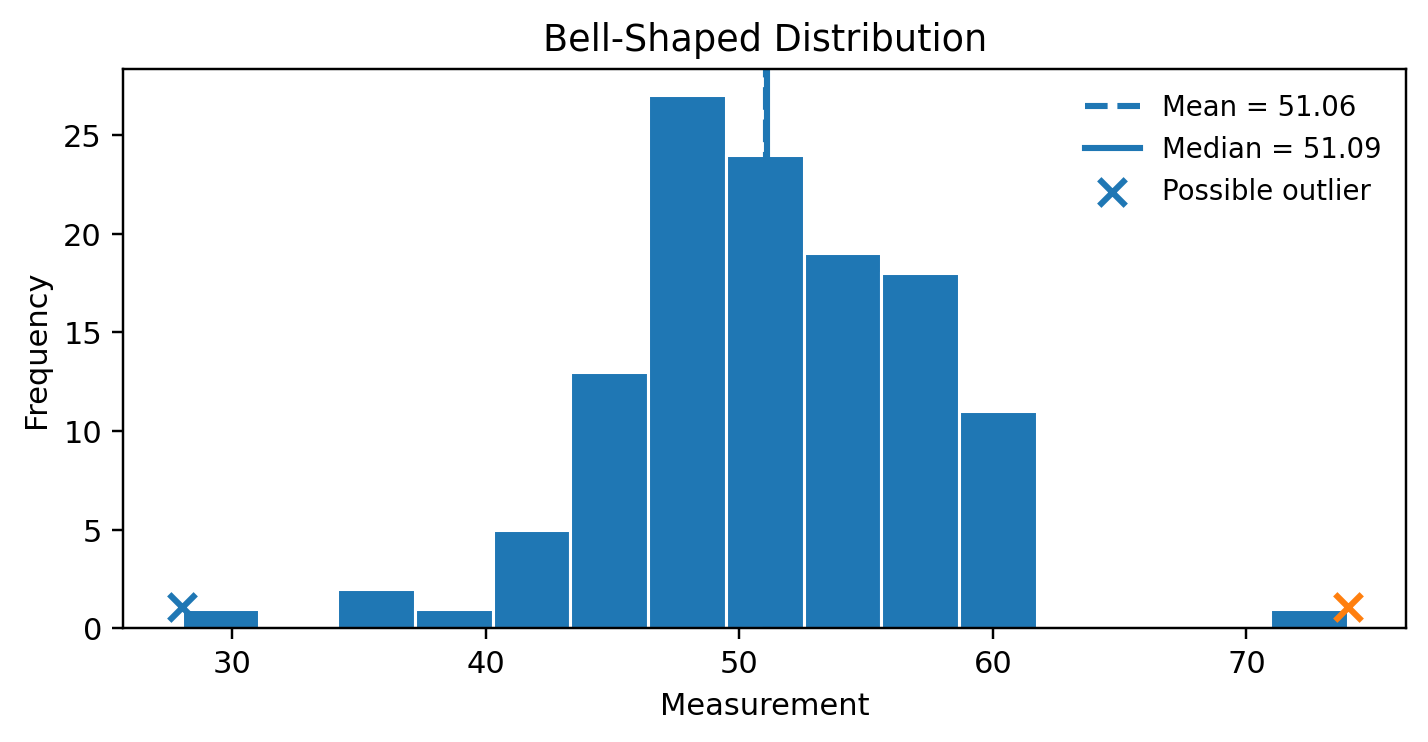
\includegraphics[width=0.52\textwidth]{fig_ch2_bell_outliers.png}
\end{center}
\scriptsize
\begin{itemize}
    \item In a roughly symmetric bell-shaped distribution, the mean and median are usually close.
    \item Most observations are concentrated near the center, but some values can still fall far from the main group.
    \item The $1.5\times IQR$ rule determines whether an extreme value is flagged as a suspected outlier.
\end{itemize}
\end{frame}

% SLIDE 32
\begin{frame}{Possible Outliers in Skewed Distributions}
\begin{columns}[T]
    \begin{column}{0.49\textwidth}
        \begin{center}
            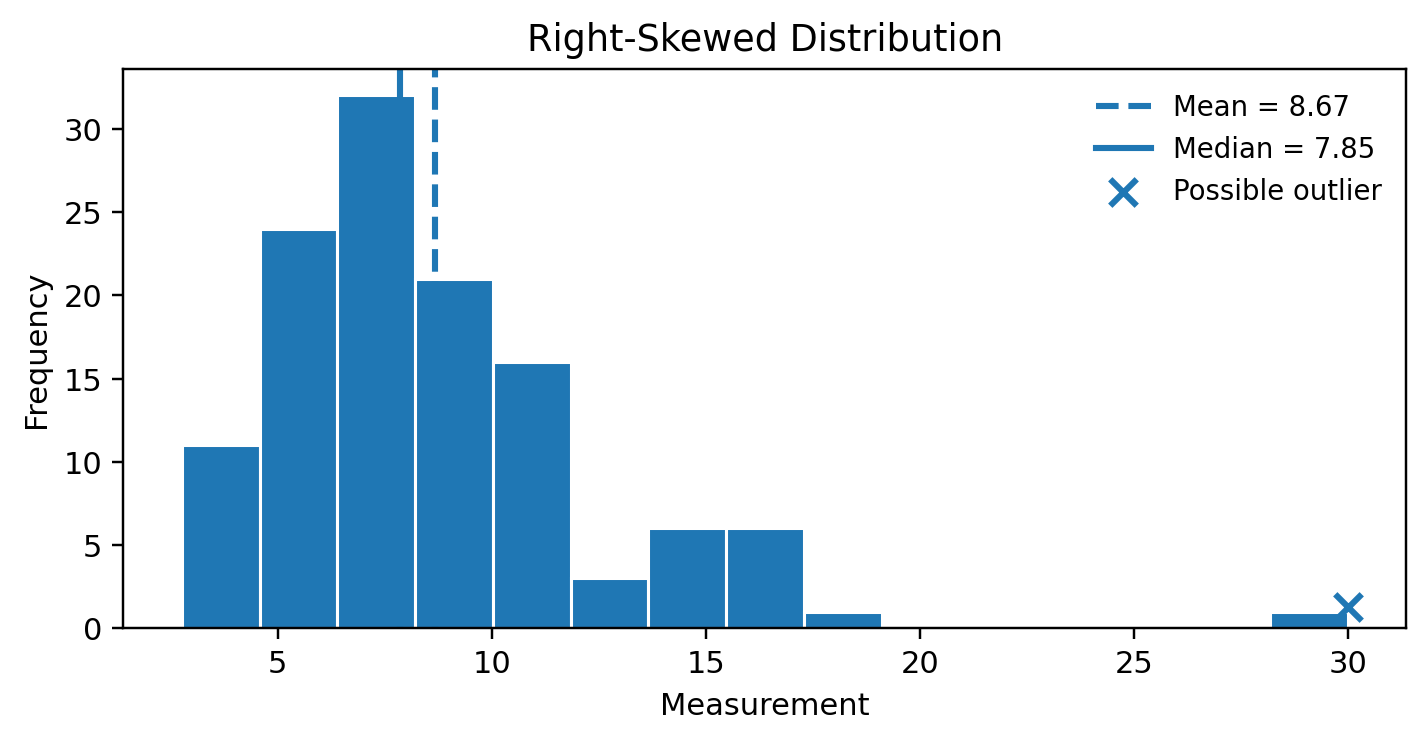
\includegraphics[width=0.84\textwidth]{fig_ch2_right_skew_outliers.png}
        \end{center}
        \scriptsize
        A right-skewed distribution has a long right tail. The mean is usually larger than the median. A suspected outlier may occur far into the upper tail.
    \end{column}

    \begin{column}{0.49\textwidth}
        \begin{center}
            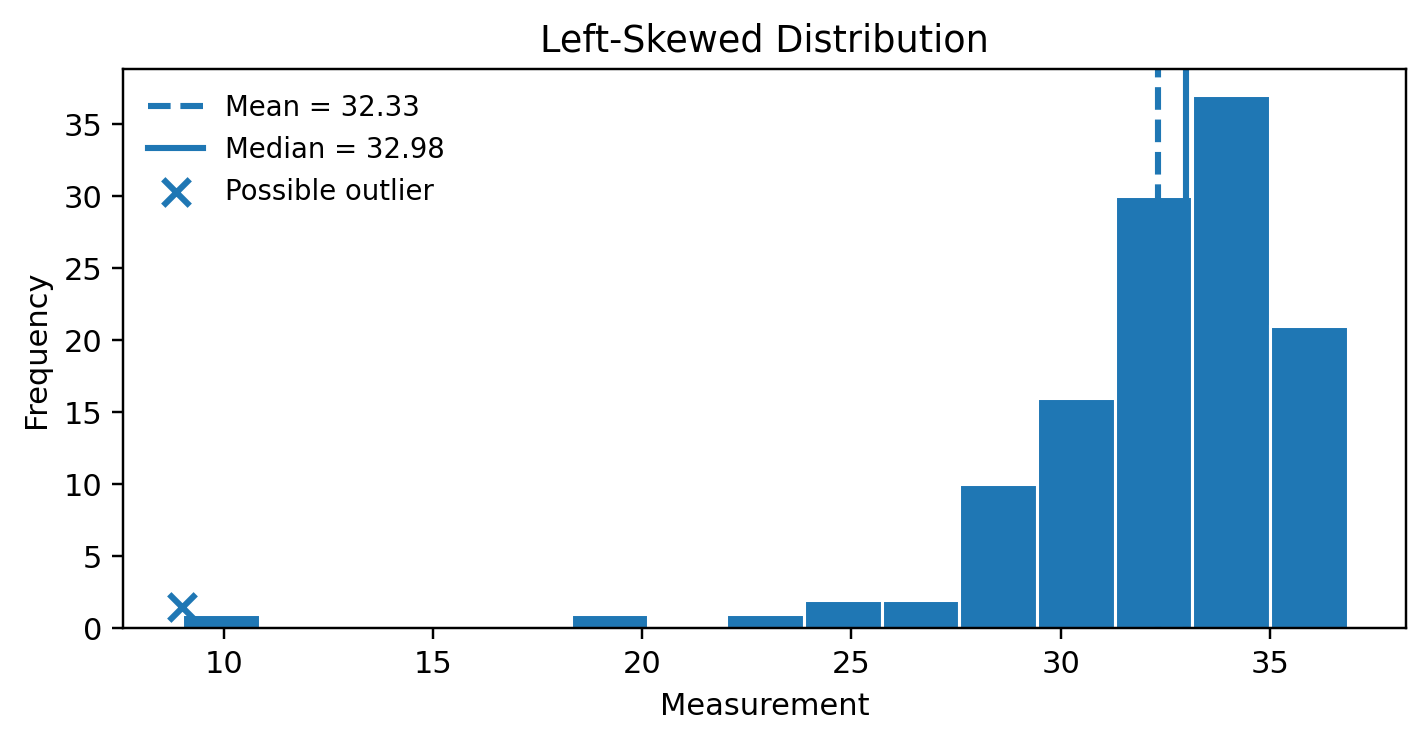
\includegraphics[width=0.84\textwidth]{fig_ch2_left_skew_outliers.png}
        \end{center}
        \scriptsize
        A left-skewed distribution has a long left tail. The mean is usually smaller than the median. A suspected outlier may occur far into the lower tail.
    \end{column}
\end{columns}

\begin{alertblock}{Important}
\scriptsize
Skewness alone does not make an observation an outlier. The $1.5\times IQR$ rule determines whether an observation is flagged as a suspected outlier.
\end{alertblock}
\end{frame}

% SLIDE 33
\begin{frame}[fragile]{Calculating the IQR in R}
R has a built-in function to instantly calculate the exact Interquartile Range.
\vspace{0.3cm}
\begin{block}{R Code}
\begin{verbatim}
IQR(pine_needles)
\end{verbatim}
\end{block}
\textbf{Output:}
\texttt{[1] 1.95}
\vspace{0.3cm}
\emph{Note: R uses its default quartile algorithm to compute this, so $10.55 - 8.60 = 1.95$.}
\end{frame}

% SLIDE 34
\begin{frame}{The Five-Number Summary}
By combining our measures of center, our measures of spread, and the absolute extremes of our data, we get a highly efficient snapshot of the entire distribution called the \textbf{five-number summary}:
\vspace{0.4cm}
\begin{center}
\Large $\text{Minimum} \quad Q_1 \quad \text{Median} \quad Q_3 \quad \text{Maximum}$
\end{center}
\vspace{0.4cm}
These five numbers offer a reasonably complete mathematical description of a dataset's center and spread.
\end{frame}

% SLIDE 35
\begin{frame}{Boxplots: Visualizing the Five-Number Summary}
\begin{columns}[c]
\begin{column}{0.5\textwidth}
	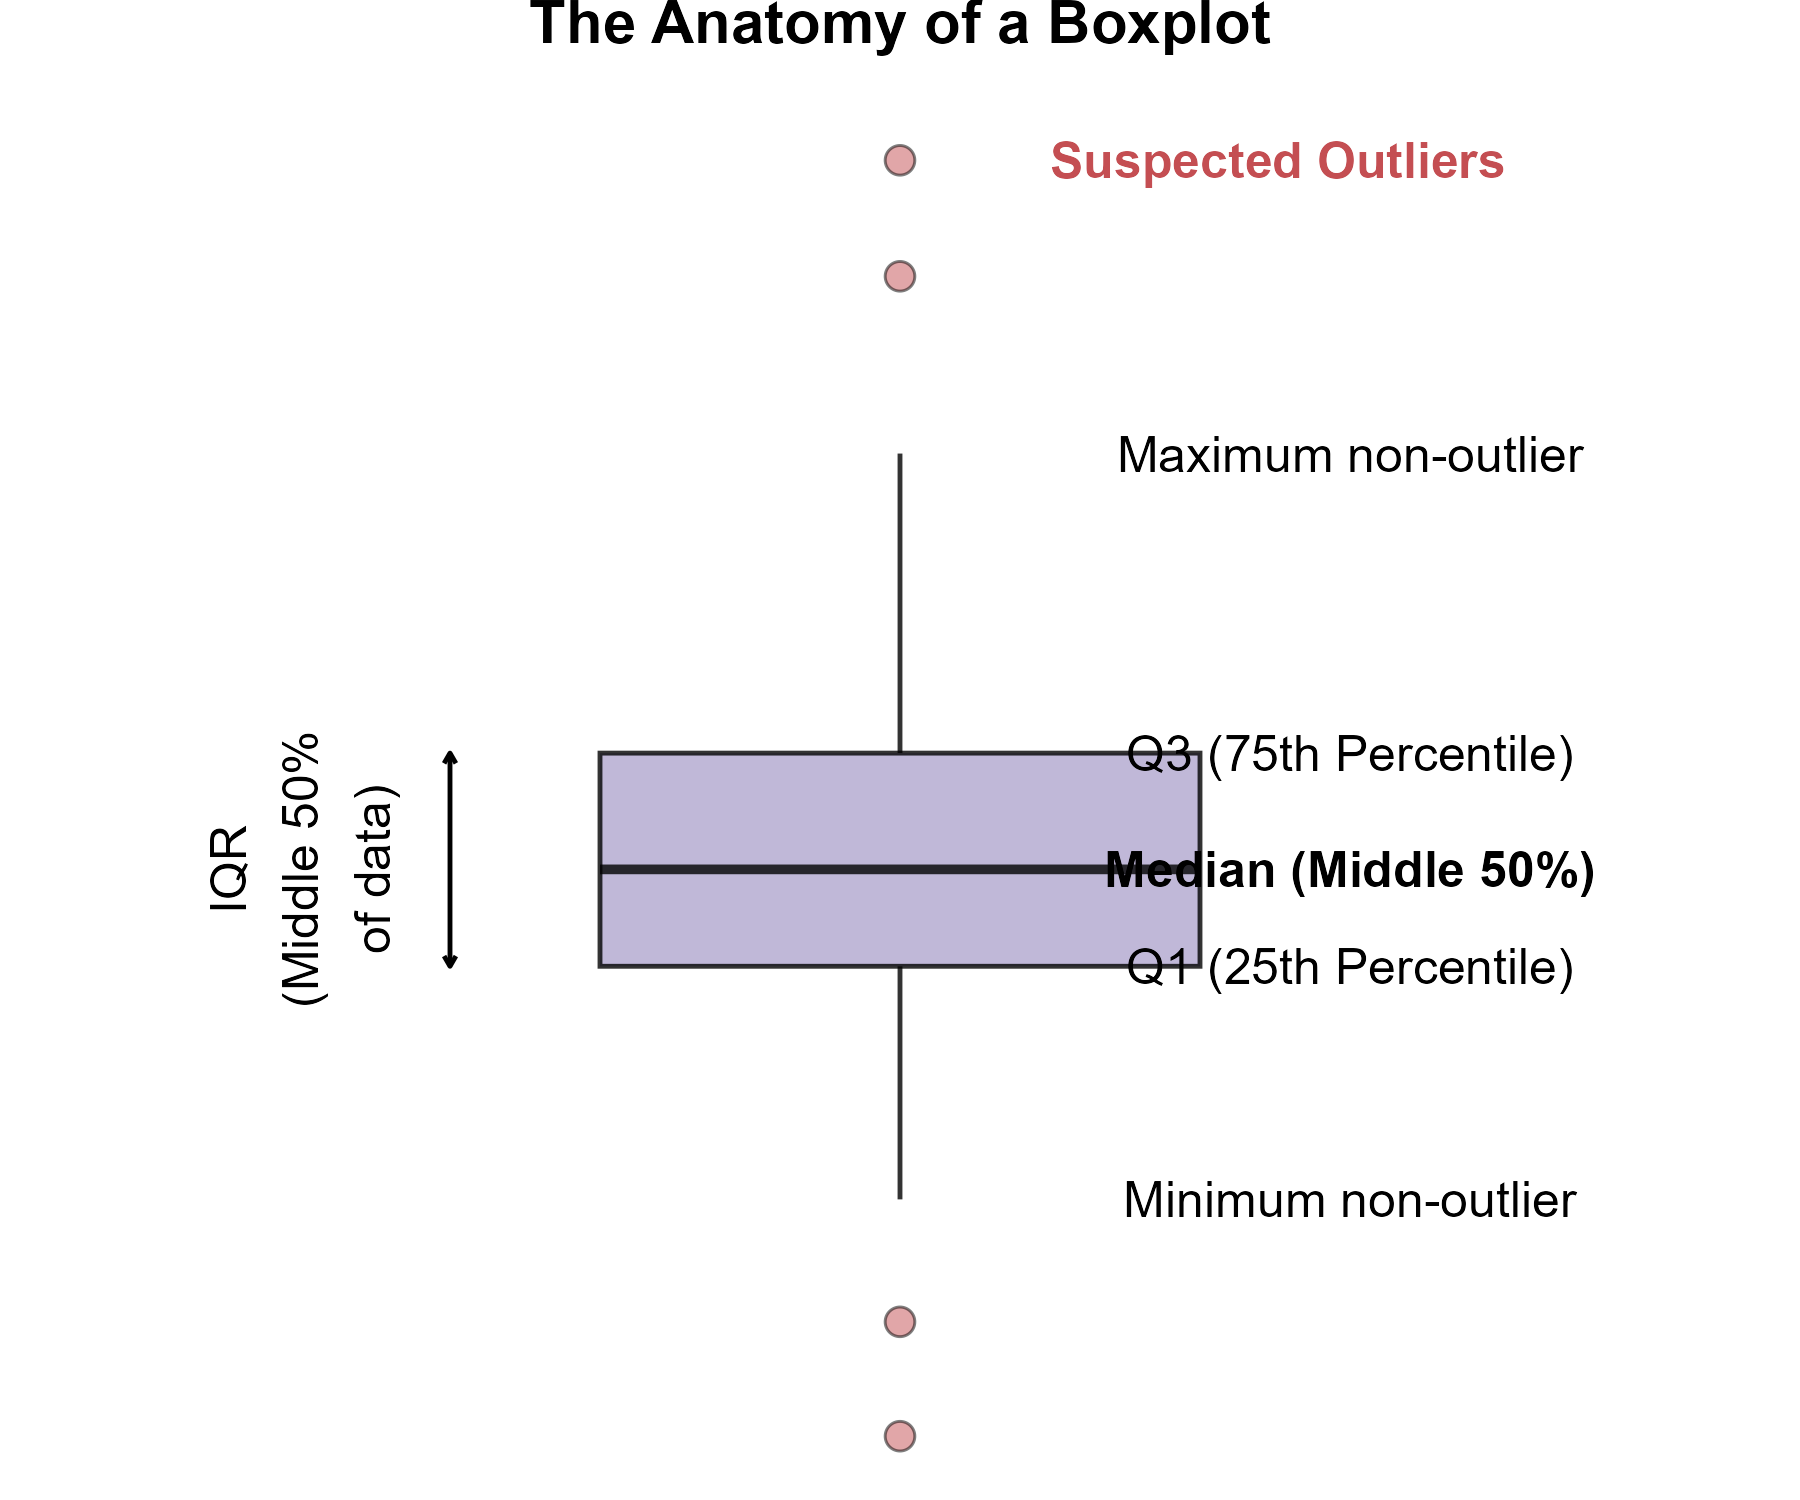
\includegraphics[width=\textwidth]{fig_ch2_boxplot_anatomy.png}
\end{column}

\begin{column}{0.48\textwidth}
\textbf{How to Read a Boxplot:}
\begin{itemize}
	\item \textbf{Box:} Spans from $Q_1$ to $Q_3$. Its width is the exact \textbf{IQR} (middle 50\%).
	\item \textbf{Thick Line:} The \textbf{Median}.
	\item \textbf{Whiskers:} Extend to the smallest and largest observations \emph{that are not considered outliers}.
	\item \textbf{Dots:} Suspected \textbf{outliers} floating beyond the whiskers.
\end{itemize}
\end{column}
\end{columns}
\end{frame}

% SLIDE 36
\begin{frame}{Side by Side Comparisons}
\begin{columns}[c]
\begin{column}{0.5\textwidth}
	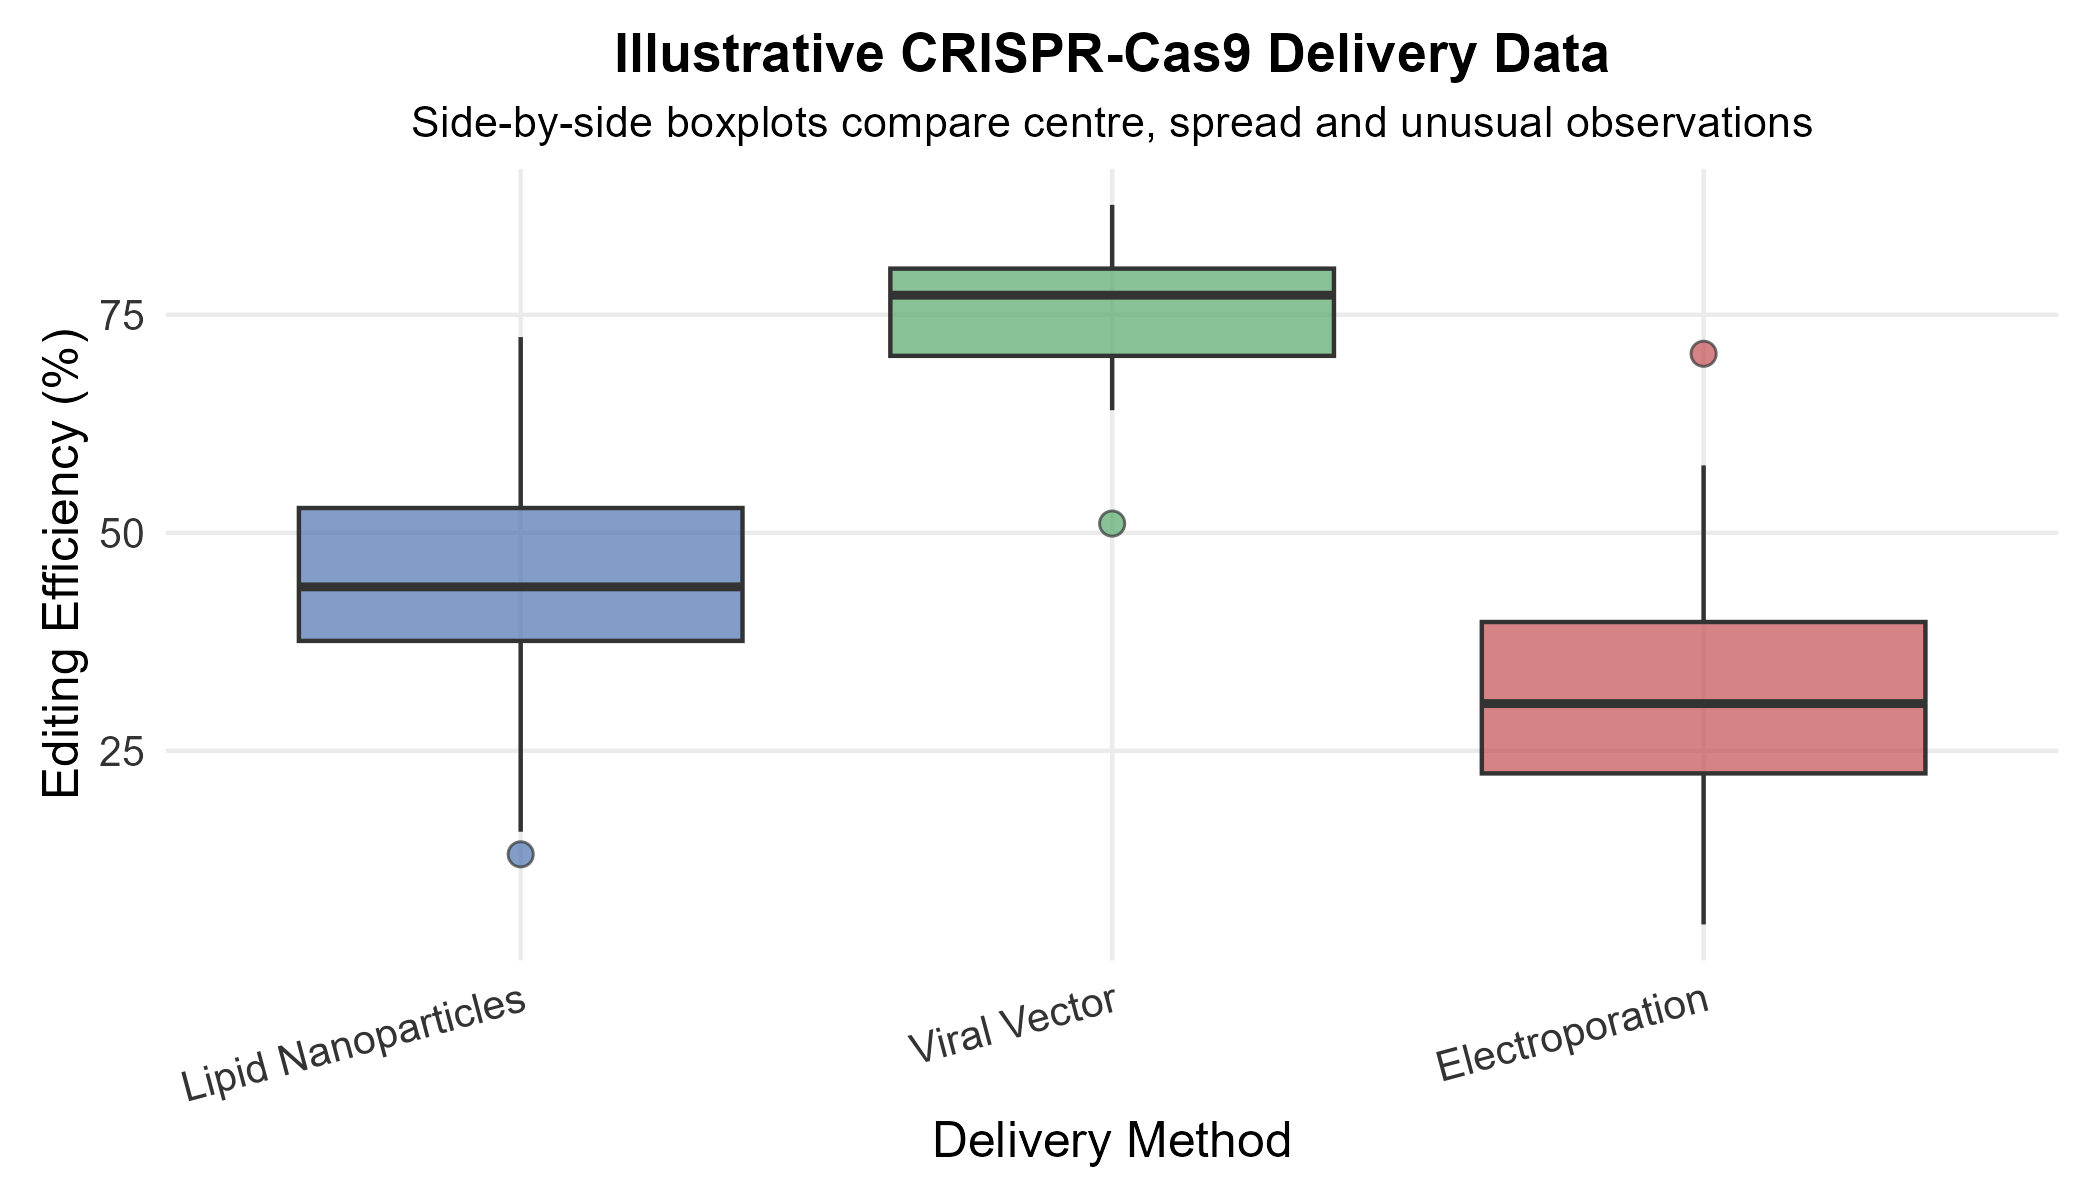
\includegraphics[width=\textwidth]{fig_ch2_side_by_side_boxplots.png}
\end{column}
\begin{column}{0.48\textwidth}
Why are boxplots so popular? They allow us to compare dozens of groups cleanly in a single graphic.
\begin{itemize}
	\item \textbf{Center:} Viral vectors yield the highest median efficiency.
	\item \textbf{Spread:} Electroporation is highly unstable (tall IQR box).
	\item \textbf{Outliers:} Lipid nanoparticles are consistent but have two high-performing outliers.
\end{itemize}
\end{column}
\end{columns}
\end{frame}

% SLIDE 37
\begin{frame}{Identifying Outliers: The $1.5 \times IQR$ Rule}
In Chapter 1, we said an outlier is an observation that falls "well outside" the overall pattern. But how does \textbf{R} automatically know which dots to plot outside the whiskers?
\vspace{0.3cm}
Statisticians use an objective mathematical formula called the \textbf{$1.5 \times IQR$ Rule}.
\vspace{0.2cm}
\begin{table}
\centering
\begin{tabular}{ll}
\toprule
\textbf{Boundary} & \textbf{Formula} \\
\midrule
\textbf{Upper Fence} & $Q_3 + (1.5 \times IQR)$ \\
\textbf{Lower Fence} & $Q_1 - (1.5 \times IQR)$ \\
\bottomrule
\end{tabular}
\end{table}
\vspace{0.2cm}
Any data point larger than the Upper Fence or smaller than the Lower Fence is plotted as an individual dot.
\end{frame}

% SLIDE 38
\begin{frame}{Break Time}
    \begin{center}
        
\includegraphics[width=0.6\textwidth]{meme_1.jpg}
    \end{center}
\end{frame}

% =============================================================
% PART V: MEASURING SPREAD (STANDARD DEVIATION)
% =============================================================

% SLIDE 39
\begin{frame}{Measuring Spread: The Standard Deviation ($s$)}
If we use the Median to measure centre, we use the IQR to measure spread. But if we use the \textbf{Mean ($\bar{x}$)} to measure center, we need a different measure of spread: \textbf{Standard Deviation ($s$)}.
\vspace{0.3cm}
\begin{columns}[c]
\begin{column}{0.48\textwidth}
\begin{itemize}
	\item The standard deviation measures spread by looking at how far each observation falls from the mean. 
	\item Conceptually, think of it as the \textbf{``average distance''} of all data points from the center.
\end{itemize}
\end{column}
\begin{column}{0.5\textwidth}
	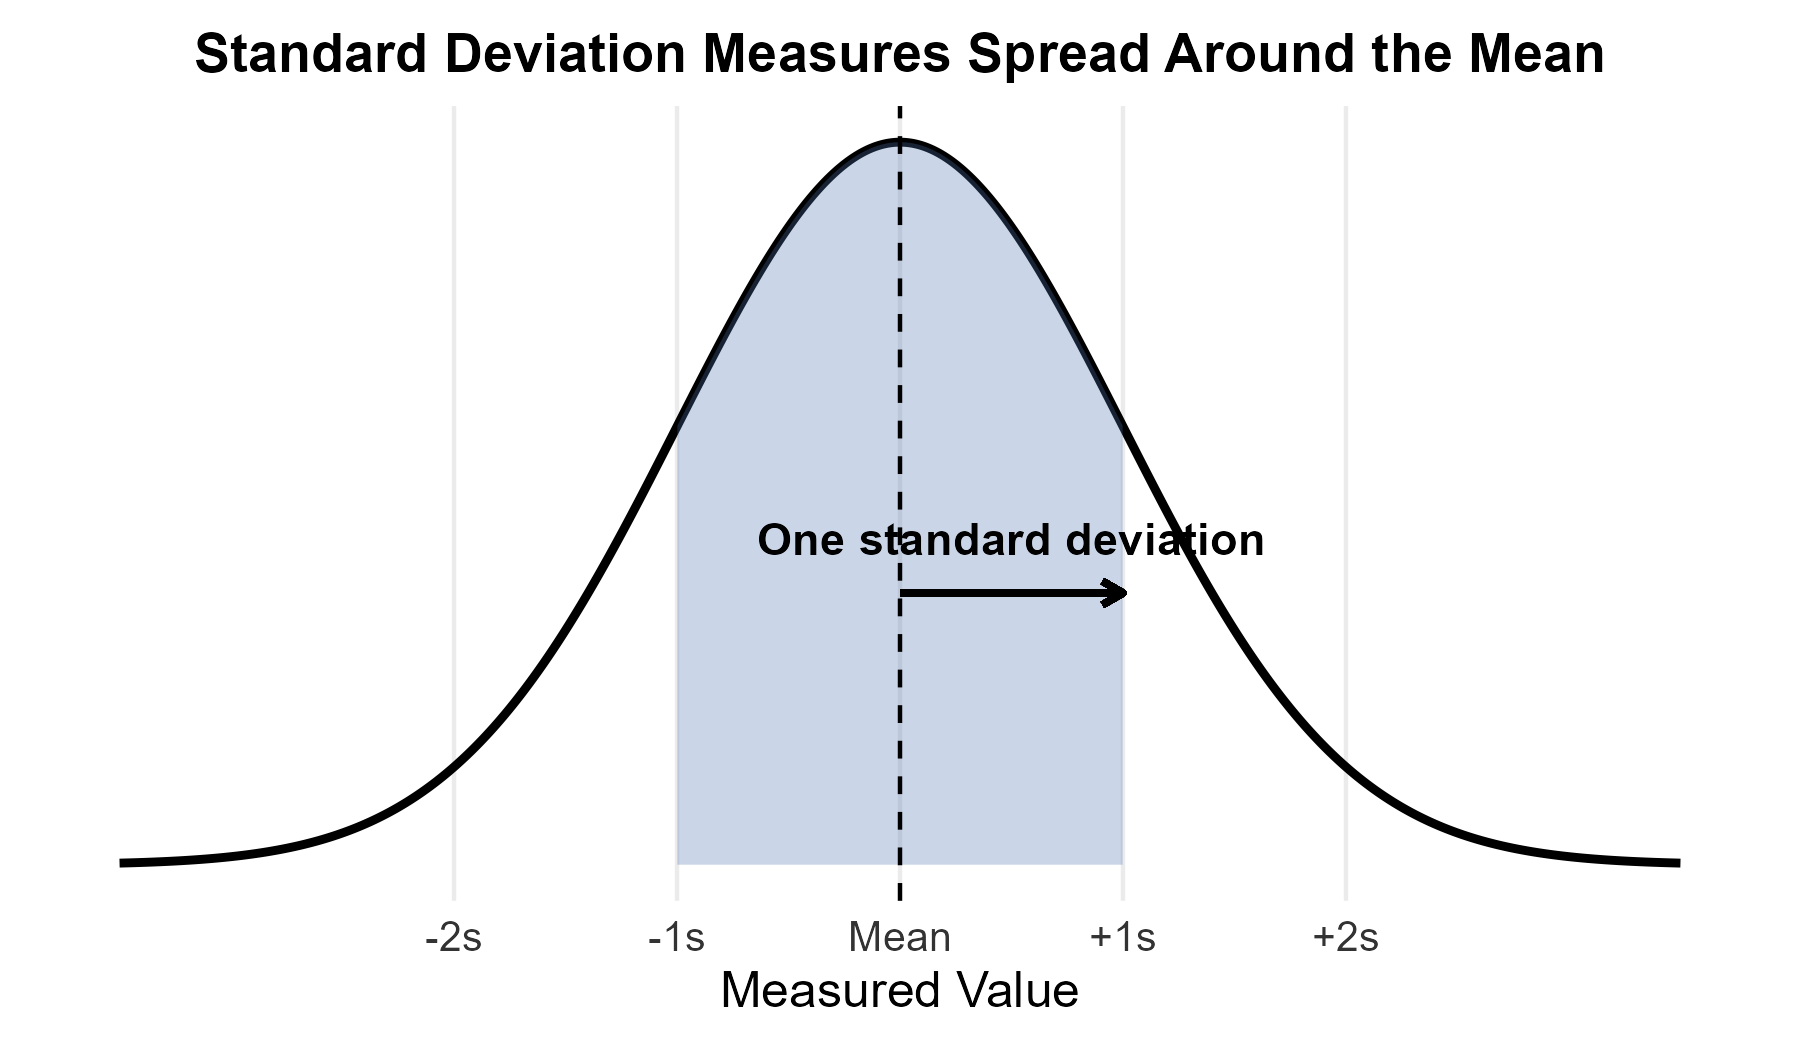
\includegraphics[width=\textwidth]{fig_ch2_standard_deviation.png}
\end{column}
\end{columns}
\end{frame}

% SLIDE 40
\begin{frame}{The Math Behind Standard Deviation}
To calculate how far the data is spread out, we find the deviation of each point: $(x_i - \bar{x})$. 
\vspace{0.2cm}
\begin{itemize}
	\item \emph{Problem:} If we just added these up, negative distances would cancel out positive distances, summing to exactly zero.
	\item \emph{Solution:} We \textbf{square} the distances to make them positive, average them, and then take the \textbf{square root} to return to original biological units.
\end{itemize}
\vspace{0.2cm}
\textbf{Variance ($s^2$)}
$$ s^2 = \frac{1}{n-1} \sum (x_i - \bar{x})^2 $$
\textbf{Standard Deviation ($s$)}
$$ s = \sqrt{\frac{1}{n-1} \sum (x_i - \bar{x})^2} $$
\end{frame}

% SLIDE 41
\begin{frame}{Degrees of Freedom: Why $(n-1)$?}
\textbf{Why do we divide by $(n-1)$ instead of $n$?}
\vspace{0.3cm}
\begin{itemize}
	\item This is a concept called \textbf{degrees of freedom}. 
	\item Because we already used our sample data to estimate the mean ($\bar{x}$) in the formula, we "spent" one piece of independent information. 
	\item Dividing by $(n-1)$ corrects a mathematical bias, ensuring our sample standard deviation perfectly estimates the true underlying population spread.
\end{itemize}
\end{frame}

% SLIDE 42
\begin{frame}{Example 2.7: Calculating SD (Metabolic Rates)}
A person's metabolic rate is the rate at which the body consumes energy. Here are the rates of 7 men in a dieting study (kilocalories/24-hour).
\vspace{0.2cm}
\textbf{Raw Data ($n=7$):} 1792, 1666, 1362, 1614, 1460, 1867, 1439
\vspace{0.4cm}
\textbf{Step 1: Find the Mean ($\bar{x}$)}
$$ \bar{x} = \frac{1792 + 1666 +1362 + 1614 + 1460 + 1867 + 1439}{7} = \frac{11{,}200}{7} = 1600 \text{ Cal} $$
\end{frame}

% SLIDE 43
\begin{frame}{Example 2.7: Find Deviations and Square Them}
Subtract the mean (1600) from every observation and square the result.
\vspace{0.2cm}
\begin{table}
\centering
\scriptsize
\begin{tabular}{crr}
\toprule
\textbf{Observation ($x_i$)} & \textbf{Deviation ($x_i - \bar{x}$)} & \textbf{Squared Deviation $(x_i - \bar{x})^2$} \\
\midrule
1792 & $1792 - 1600 = 192$ & $192^2 = 36864$ \\
1666 & $1666 - 1600 = 66$ & $66^2 = 4356$ \\
1362 & $1362 - 1600 = -238$ & $(-238)^2 = 56644$ \\
1614 & $1614 - 1600 = 14$ & $14^2 = 196$ \\
1460 & $1460 - 1600 = -140$ & $(-140)^2 = 19600$ \\
1867 & $1867 - 1600 = 267$ & $267^2 = 71289$ \\
1439 & $1439 - 1600 = -161$ & $(-161)^2 = 25921$ \\
\midrule
& \textbf{Sum = 0} & \textbf{Sum of Squares = 214870} \\
\bottomrule
\end{tabular}
\end{table}
\vspace{0.1cm}
\emph{Notice the un squared deviations sum to exactly zero!}
\end{frame}

% SLIDE 44
\begin{frame}{Example 2.7: Calculate Variance and SD}
\textbf{Step 3: Calculate Variance ($s^2$)} \\
Divide the sum of squared deviations by $n - 1$ (which is $7 - 1 = 6$)
$$ s^2 = \frac{214870}{6} = 35811.67 \text{ Cal}^2 $$
\vspace{0.3cm}
\textbf{Step 4: Calculate Standard Deviation ($s$)} \\
Take the square root of the variance to return to the original units:
$$ s = \sqrt{35811.67} = 189.24 \text{ Cal} $$
\vspace{0.3cm}
\textbf{Conclusion:} The men burn an average of \textbf{1600 Cal} per day and their rates typically vary from that mean by about \textbf{189.24 Cal}.
\end{frame}

% SLIDE 45
\begin{frame}[fragile]{Example 2.7: Calculating Variance and SD in R}
\begin{block}{R Code}
\begin{verbatim}
# Create a vector of the 7 metabolic rates
metabolic_rates <- c(1792, 1666, 1362, 1614, 1460, 1867, 1439)

# Calculate Variance (s^2)
var(metabolic_rates)

# Calculate Standard Deviation (s)
sd(metabolic_rates)
\end{verbatim}
\end{block}
\textbf{Output:}
\begin{verbatim}
[1] 35811.67
[1] 189.2397
\end{verbatim}
\end{frame}

% SLIDE 46
\begin{frame}{Properties of the Standard Deviation}
\begin{itemize}
	\item \textbf{Measures spread around the mean:} It should only be used when $\bar{x}$ is chosen as the measure of center.
	\item Always \textbf{$s \ge 0$:} $s = 0$ only when there is zero spread (all observations are identical). Otherwise, $s > 0$.
	\item \textbf{Same units as original data:} For example, f you measure tumor diameter in millimeters (mm), $s$ is in mm. (Variance is in mm$^2$, which is biologically unhelpful).
	\item \textbf{Non resistant!} Because the formula uses the mean and squares the distances, a single extreme outlier will inflate $s$ drastically.
\end{itemize}
\end{frame}

% =============================================================
% PART VI: CHOOSING THE RIGHT SUMMARY & SYNTHESIS
% =============================================================

% SLIDE 47
\begin{frame}{Choosing the Right Summary}
You now have two complete sets of tools to summarize a quantitative distribution. How do you choose? It depends entirely on \textbf{Shape} and \textbf{Outliers}.
\vspace{0.2cm}
\begin{table}
\centering
\small
\begin{tabular}{p{2cm}p{4cm}p{4cm}}
\toprule
\textbf{When to Use} & \textbf{Mean \& Standard Dev.} & \textbf{Median \& IQR (5-Number)} \\
\midrule
\textbf{Shape} & Reasonably Symmetric & Skewed (Left or Right) \\
\textbf{Outliers} & No extreme outliers & Contains suspected outliers \\
\textbf{Why?} & \textbf{Non-resistant.} Powerful for normal biology, but easily ruined by extreme values. & \textbf{Resistant.} Provides a stable snapshot even when outliers are present. \\
\bottomrule
\end{tabular}
\end{table}
\end{frame}

% SLIDE 48
\begin{frame}[fragile]{Summary of R Commands (Chapter 2)} 
Here are the key functions introduced in this chapter for calculating numerical summaries of a dataset (vector) \texttt{x}:
\begin{table}
\centering
\small
\begin{tabular}{lp{8.5cm}}
\toprule
\textbf{R Command} & \textbf{What it Calculates} \\
\midrule
\texttt{c(1, 2, 3)} & Combines individual data values into a single vector. \\
\addlinespace
\texttt{mean(x)} & Calculates the sample mean ($\bar{x}$) \\
\addlinespace
\texttt{median(x)} & Calculates the exact median ($M$) \\
\addlinespace
\texttt{summary(x)} & Outputs the five number summary (Minimum, $Q_1$, Median, $Q_3$, Maximum) plus the mean \\
\addlinespace
\texttt{IQR(x)} & Calculates the Interquartile Range ($Q_3 - Q_1$) \\
 \addlinespace
\texttt{var(x)} & Calculates the sample variance ($s^2$) \\
\addlinespace
\texttt{sd(x)} & Calculates the sample standard deviation ($s$) \\
\bottomrule
\end{tabular}
\end{table}
\end{frame}

% SLIDE 49
\begin{frame}{What’s Next? Looking Ahead to Chapter 3}
\begin{itemize}
	\item In Chapters 1 and 2, we explored data that had only \textbf{one variable} recorded per individual.
	\item However, we often want to know if two different variables are connected.
	\begin{itemize}
	      \item \emph{Does a higher dosage of a drug cause a faster drop in blood pressure?}
	      \item \emph{Is a specific genetic mutation linked to a higher risk of heart disease?}
	\end{itemize}
	\item In \textbf{Chapter 3: Scatterplots and Correlation}, we will learn how to visualize and mathematically measure the relationship between \textbf{two quantitative variables} measured on the same individual.
 \end{itemize}
\end{frame}

\end{document}
